\documentclass[runningheads]{llncs}
\usepackage{graphicx}
\usepackage{amsmath,amssymb} % define this before the line numbering.
\usepackage{ruler}
\usepackage{color}
\usepackage[width=122mm,left=12mm,paperwidth=146mm,height=193mm,top=12mm,paperheight=217mm]{geometry}
\begin{document}
% \renewcommand\thelinenumber{\color[rgb]{0.2,0.5,0.8}\normalfont\sffamily\scriptsize\arabic{linenumber}\color[rgb]{0,0,0}}
% \renewcommand\makeLineNumber {\hss\thelinenumber\ \hspace{6mm} \rlap{\hskip\textwidth\ \hspace{6.5mm}\thelinenumber}}
% \linenumbers
\pagestyle{headings}

% Command definitions
\def\subsectionautorefname{section}
\definecolor{light-gray}{gray}{0.3}
\newcommand{\aside}[1]{\textcolor{light-gray}{\emph{#1}}}
\newcommand{\comment}[1]{}

\mainmatter
\def\ECCV12SubNumber{***}  % Insert your submission number here

\title{Timely Object Detection}

\titlerunning{ECCV-12 submission ID \ECCV12SubNumber}

\authorrunning{ECCV-12 submission ID \ECCV12SubNumber}

\author{Anonymous ECCV submission}
\institute{Paper ID \ECCV12SubNumber}

\maketitle

\begin{abstract}
\end{abstract}

\section{Sequential Decision Problem} \label{sec:sdp}

We first describe the requirements for our target system, and set the notation.
Details of our implementation are then given.

We deal with a dataset of images $\mathcal{D}$, where each image $\mathcal{I}$ contains at least one, and often multiple, objects.
Each object is labeled with exactly one category label $1$ through $K$.

The multi-class, multi-label \emph{classification} problem asks whether $\mathcal{I}$ contains at least one object of class $i$, for each class $i \in \{1,\dots,K\}$.
The answer for a single label is given with a real-valued confidence by a function $\emph{classify}(I,i)$.
We write the ground truth for an image as $\mathbf{C}=\{C_1,\dots,C_K\}$, where $C_i$ is a $\{0/1\}$ binary variable set to $1$ if an object of class $i$ is present.
Henceforth we write $P(C_i)$ to mean $P(C_i=1)$, as shorthand.

The answer is evaluated by plotting precision vs. recall across dataset $\mathcal{D}$ (by progressively lowering the confidence threshold for a positive label) and integrating to yield the Average Precision (AP) metric \cite{pascal-voc-2010}.

We can make the classification problem more difficult by posing the \emph{counting} problem, which asks how many objects of class $i$ are present in $\mathcal{I}$, for each $i$.
This setting is not commonly evaluated; we mention it for its usefulness in later exposition.

Finally, the \emph{detection} problem is to output a list of bounding boxes (sub-images defined by four coordinates), each with a real-valued confidence that it encloses a single instance of an object of class $i$.
The answer for a single class $i$ is given by an algorithm $\emph{detect}(\mathcal{I},i)$, which outputs a list of bounding boxes $B$ and associated confidences.
To highlight the hierarchical structure of these problems, we note that the confidences may be given by $\operatorname{classify}(b,i)$ for each sub-image $b \in B$, and that the correct answer to the detection problem also answers the counting and classification problems.

Here we describe the classification problem setup, although we evaluate performance on both classification and detection tasks.

\subsection{Multi-class Classification Policy}

Our goal is a multi-class classification policy $\pi$ that takes an image $\mathcal{I}$ and outputs $\{\emph{classify}(C_1), \dots, \emph{classify}(C_K)\}$, where we omit the obvious dependency on $\mathcal{I}$.
The policy repeatedly selects an action $a$ from a set of actions $\mathcal{A}$, executes it, potentially receiving a set of observations, and selects the next action.
A dynamic (or ``closed-loop'') policy bases action selection on observations received from previous actions, allowing context to play a large role.
This sets our problem formulation apart from multi-class systems that evaluate in a fixed order, such as simple cascades \cite{Viola2001}.

The set of actions $\mathcal{A}$ can include per-class classifiers, ``scene context'' functions, and feature computations.
For simplicity of exposition, let $\mathcal{A}$ consist of $2$ feature computations $F$ and $2K$ per-class classifiers $L$:
\begin{itemize}
	\item $L^\text{co}$ are one-vs-all SVMs on a complex featurization of the image (computed by $F^\text{co}$);
	\item $L^\text{sc}$ are SVMs on a simple scene-level feature (computed by $F^\text{sc}$).
\end{itemize}

Each classifier $L$ or feature computation $F$ has an expected cost of execution.
Depending on the setting, the cost can be defined in terms of algorithmic runtime analysis (e.g. $O(N^3)$), an idealized property such as number of \emph{flops}, or simply the empirical runtime on specific hardware.
We take the empirical approach: every executed action advances $t$, the \emph{time into episode}, by its empirical runtime.

The system is given two times: the setup time $T_s$ and deadline $T_d$.
Between these times, the system must meet the goal of \emph{Anytime} performance and give the best possible answer at any point.

\begin{figure}[h!]
\center{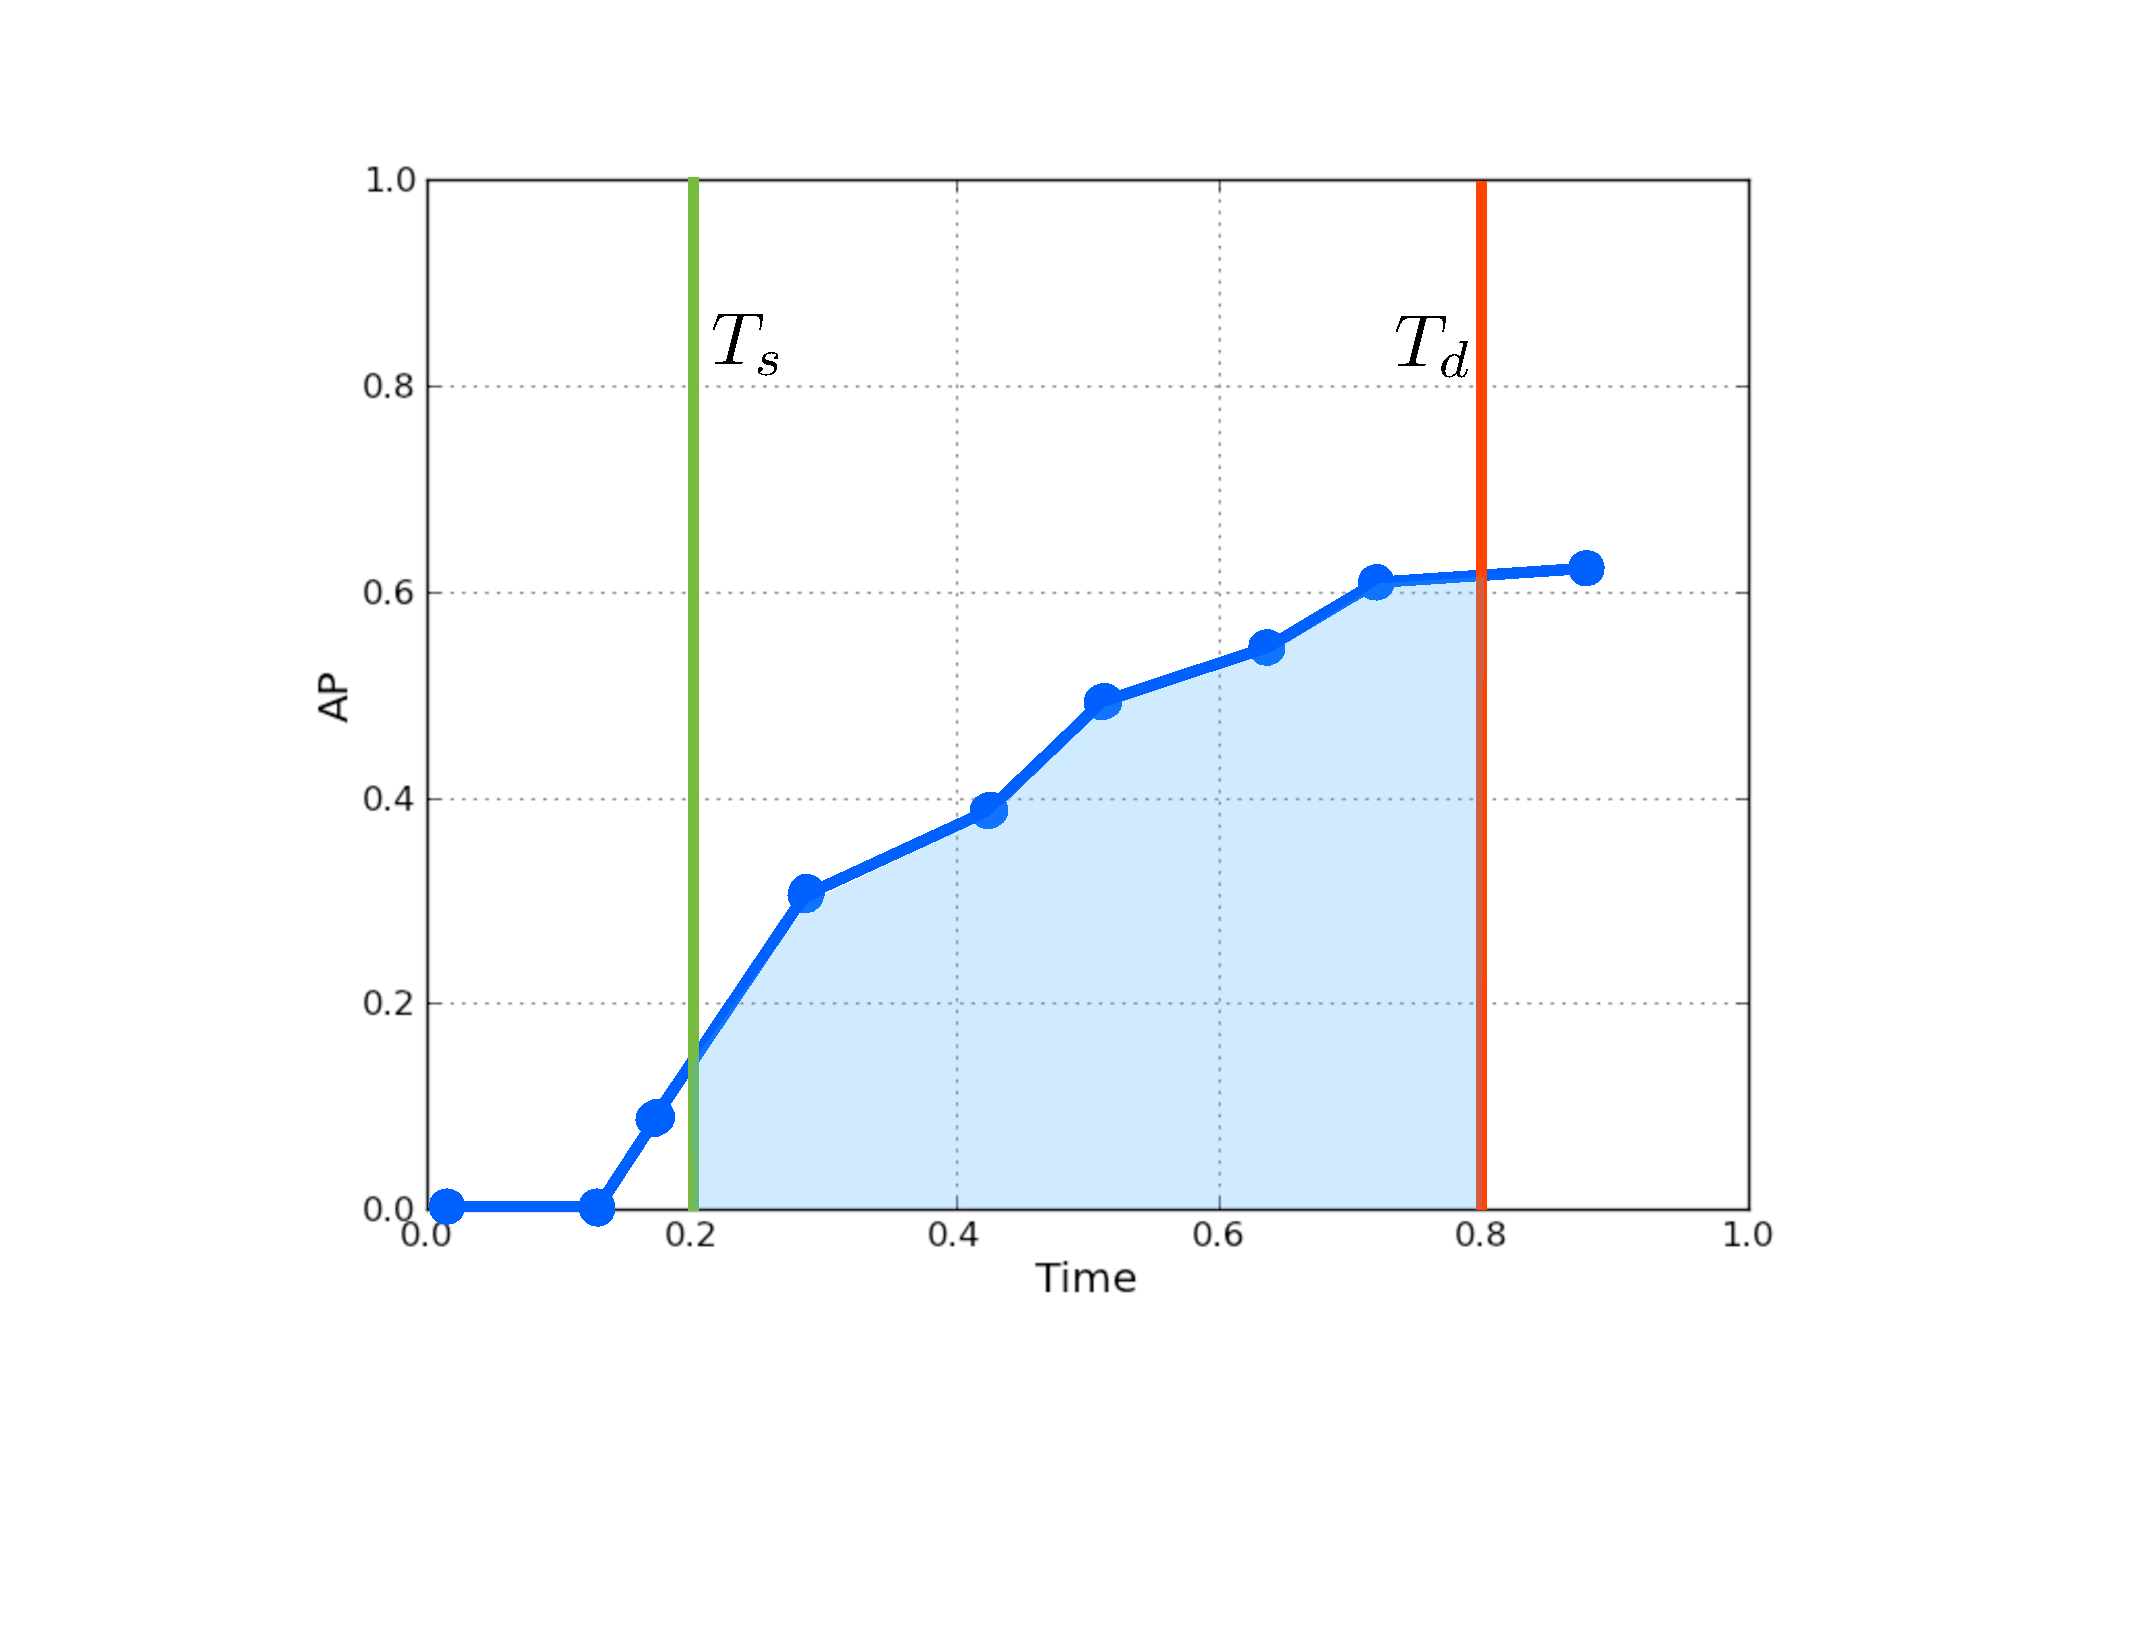
\includegraphics[width=0.66\linewidth]
    {figures/evaluation.pdf}}
  \caption{\label{fig:evaluation}Our objective is to obtain \emph{Anytime} performance within the bounds of the curve. That is, the policy should give the best possible answer at any time from start time to deadline.}
\end{figure}

To meet this goal, the evaluation metric of a policy is defined as the area under the performance vs. time curve between points $T_s$ and $T_d$ (see Figure~\ref{fig:evaluation}).
We evaluate policies by this more robust metric and not simply by the final performance at deadline time for the same reason---robustness---that Average Precision is used instead of a fixed Precision vs. Recall point.

In the language of decision processes, we define the \emph{state} of the decision process by the setting of $\mathbf{C}$ (the $K$ object presence variables $C_i$) and the time into episode $t$.
When the state has all the necessary information to make optimal action selections, the problem can be formalized as a Markov Decision Process.
Obviously, the true value of $\mathbf{C}$ is unknown to our system, so we define a \emph{belief state} $b$ as a distribution over states.
The belief state consists of the distribution $P(\mathbf{C}) = P(C_1, \dots, C_K)$, as well as $t$, and other variables.

A classification \emph{episode} takes an image $\mathcal{I}$ and proceeds from the initial belief state $b_0$ and action $a_0$ to the next pair $(b_1,a_1)$ and so on until $t$ exceeds $T_d$.
At that point, the policy is terminated and a new episode begins on a new image.

\begin{table}
\centering
\caption{Summary of the notation used.}
\label{tab:notation}
\begin{tabular}{|l|l|}
	\hline
	$C_i$         & presence of at least one object of class $i$  \\ 
	$K$           & number of object classes                      \\ 
	$t$           & time into episode                             \\ 
	$T_s$, $T_d$  & start and deadline times                      \\ 
	$\mathcal{A}$ & set of actions                                \\ 
	$b_j$        	& belief state at step $j$                                 \\ 
	$\pi$         & policy, $\phi(b_s) \mapsto a \in \mathcal{A}$ \\ 
	\hline
\end{tabular}\end{table}

\subsection{Reward definition}
Optimal performance results from becoming maximally certain of the correct values of every $C_i$ as quickly as possible (given the setup time).
Toward this goal, we formulate a \emph{reward function} that encourages this behavior by assigning a score to an action taken in a belief state.
Let's say that given deadline $T_d$, the policy had time to take $J$ actions.
The total expected reward of a policy $\pi$ is then defined as the sum of rewards
\begin{equation}
\mathbb{E}_\pi[\sum_{j=0}^J R(b_j, a_j)]
\end{equation}
We explore two options for the reward function: the first is derived directly from the evaluation metric; the second cares only about entropy of $P(\mathbf{C})$.

\subsubsection{Slope of performance vs. time}
Remembering that the final evaluation of a policy consists of the area under the performance vs. time curve, we formulate a per-action reward such that the addition of 

\subsubsection{Information gain}

\subsection{Learning the value of an action}
At each step, we want to pick the action that maximizes the expected rewards until the end of the episode.

\section{Evaluation} \label{sec:evaluation}

\bibliographystyle{splncs}
\bibliography{sergeyk-bibtex}

\end{document}
